\important{Simulation}
\chapterauthor{Jayden Yanzick}
\info{Jayden Yanzick}{Simulation}{October 18, 2024}
\label{simulation}

\section*{Intro to the AI}
As AI grows into our everyday lives, so too does it grow into the field of robotics. Every year, more companies around the world digitalize into new AI models to manage their algorithms and systems more efficiently. Because of that, I would like to present my side of AI, with an AI simulator that's been in development since May of this year. Using complex algorithms and various mathematical concepts, its purpose is to create the best skills run designed for our bot and the field.

\section*{The Simulator as a Whole}
The simulator used is called Webots. It is a digital robotics simulator that allows for unlimited design possibilities, using different programming languages to control bots. In this case, I am designing a simulator containing the field, the bot, and a neural network utilizing Deep Reinforcement Learning. Webots uses \textit{Nodes} to define objects in the simulated world, which enables the bot to interact with the environment. There are many types of nodes, but I will focus only on the main ones used in our project.

\begin{figure}
    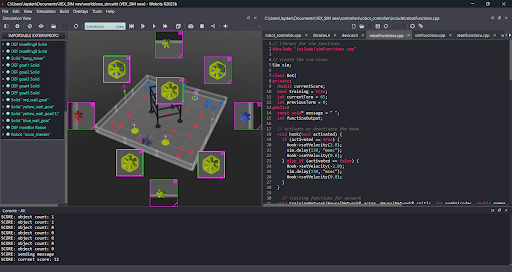
\includegraphics[width=0.9\linewidth]{images/simsoftware}
    \captionof{figure}{The Simulation Software} % Use \captionof instead of \caption
    \label{fig:simsoftware}
\end{figure}

\section*{CAD Designing and Modeling}
To design the bot inside the simulator, we use Fusion 360 to create CAD models. While Webots does offer basic shape modeling (e.g., cubes, spheres, cones), more complex parts require external CAD software. These models allow us to visualize designs in a digital environment without risking damage to the physical bot. The CAD models are optimized for memory efficiency and integrated into the simulator using Nodes. Game objects and field elements are imported directly from the CAD files provided by VEX.

\section*{Deep Reinforcement Learning and the Neural Network}
Our neural network is based on Deep Reinforcement Learning (DRL). DRL combines two concepts:  
- \textbf{Deep Learning:} Enables the network to make decisions based on the state of the field, such as the location of game objects and the bot’s position.  
- \textbf{Reinforcement Learning:} Involves multiple "episodes," where each episode is a complete skills run. The neural network learns through these repeated episodes, improving its performance by recognizing scoring opportunities and efficient strategies.

\begin{figure}
    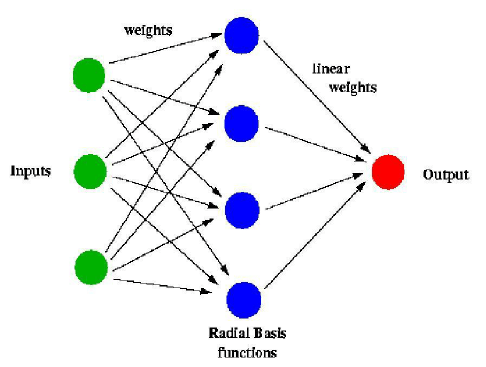
\includegraphics[width=0.9\linewidth]{images/neuralexample}
    \captionof{figure}{An example of a neural network.}
    \label{Fig:neuralexample}
\end{figure}

In the current configuration, the network consists of 4 input neurons, 512 hidden neurons, and 1 output neuron. The output determines the bot's actions. Here’s a simplified example of how the code processes the output:

\begin{verbatim}
double action = 1.0;
round(1, action * 2);
if (action == 1) {
    // movement function
}
\end{verbatim}

This code multiplies the output by 2 and rounds it to a whole number. The result triggers a specific function, which executes the desired action. The process repeats, allowing the network to learn through trial and error.

\section*{Programming the Main Bot}
The main robot is controlled through a \textit{Supervisor} node, which grants it additional capabilities. This allows the bot to manage the simulation independently. The robot’s components include:
\begin{itemize}
    \item Seven motors: Six for the drivetrain, one for a hook to grab goals.
    \item Receiver and Emitter nodes: Used for communication with other bots.
\end{itemize}

To initialize devices within Webots, you must define them in code, as shown below:

\begin{verbatim}
#include <webots/Robot.hpp>
#include <webots/Motor.hpp>

using namespace webots;

Robot *robot = new Robot();
Motor *example = robot->getMotor("example");
\end{verbatim}

The \verb|#include| statements import the required classes, enabling the creation of the robot and its components. The code is organized across multiple files, with the primary file named after the controller (e.g., \verb|<controller_name>.exe|). Devices are defined separately, while functions are organized within classes.

\begin{figure}[h]
    \centering
    \caption{The first 27 lines of initializing devices in the simulator.}
    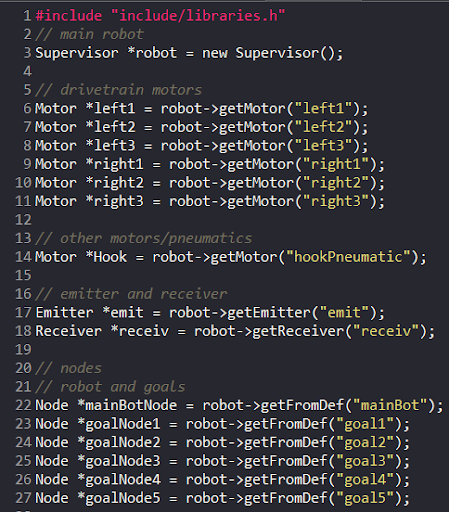
\includegraphics[width=0.9\linewidth]{images/initalizing.png}
\end{figure}

We use four classes to organize the code:
\begin{itemize}
    \item \textbf{Bot:} Contains functions for the robot.
    \item \textbf{Sim:} Manages simulation-related functions.
    \item \textbf{NeuralNetwork:} Handles the neural network’s operations.
    \item \textbf{Reset:} Manages manual resets of the simulation.
\end{itemize}

\section*{Programming the Scoring Bot}
The scoring bot operates with a separate controller, as each robot requires its own controller. It uses \textit{Camera} and \textit{Connector} nodes to track goals and count rings. The camera can detect predefined object colors, allowing the bot to calculate the score accurately. Here’s a sample of the scoring logic:

\begin{verbatim}
switch (objectCount) {
    case 1:
        currentScore += 3;
        break;
    case 2:
        currentScore += 4;
        break;
    // intervals increase by 1 for each additional ring
}
\end{verbatim}

The score is printed to the console and sent to the neural network through an Emitter node, allowing the network to adjust weights based on the run’s outcome.

\begin{figure}[h]
    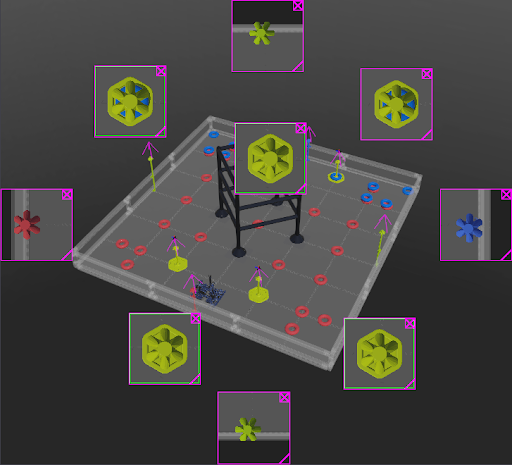
\includegraphics[width=0.9\linewidth]{images/simfield.png}
    \centering
    \caption{The field with camera overlays.}
    \label{Fig:simfield}
\end{figure}

\section*{Training the Neural Network}
Before the training begins, the two bots perform a radio check to confirm communication. The neural network then initiates random actions within the field. Once the simulation timer expires, the final score is pushed to the network, which updates the weights of the neurons. The simulator resets, and the training loop starts again for the next run.
